\chapter{Zimlet tools}

There are three points where zimlet provides new utilites:
\begin{enumerate}
    \item{A new tab in the main view (Figure \ref{fig:appTab})}
    \item{A new item in the dropdown menu of the attach button in compose view(Figure \ref{fig:attachMenu})}
    \item{A new item in the dropdown menu of the top search toolbar(Figure \ref{fig:searchMenu})}
\end{enumerate}

\begin{figure}[htbp,!h] 
\centering 

\includegraphics[scale=0.2]{\srcPath/images/ZD-appTabs.png} 
\caption{New tab} 
\label{fig:appTab}
\end{figure}
\begin{figure}[htbp,!h]
    \centering
    \begin{minipage}{0.45\textwidth}
        \centering
        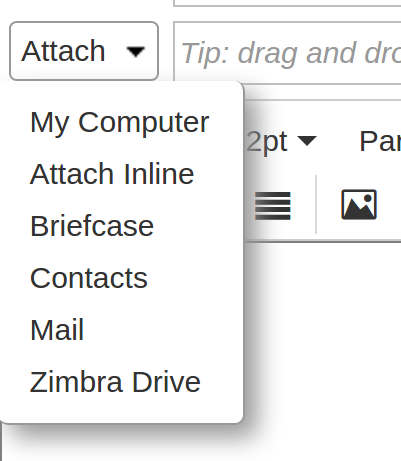
\includegraphics[width=0.5\textwidth]{\srcPath/images/ZD-attachMenu.png} % second figure itself
        \caption{Attach menu}
        \label{fig:attachMenu}
    \end{minipage}
    \hfill
    \begin{minipage}{0.45\textwidth}
        \centering
        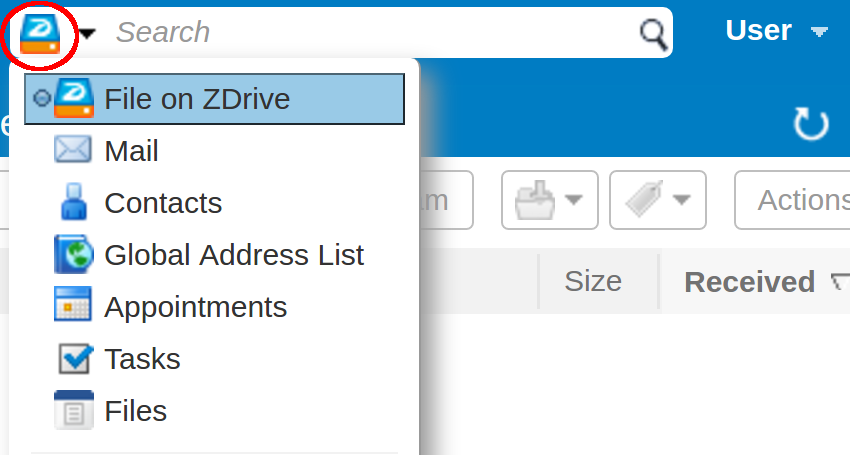
\includegraphics[width=0.9\textwidth]{\srcPath/images/ZD-searchMenu.png} % first figure itself
        \caption{Search menu}
        \label{fig:searchMenu}
    \end{minipage}
\end{figure}

\section{Drive App Tab}

The main option to interact with Drive is clicking on the Drive tab.
This click can have two different behaviours: 
\begin{itemize}
\item{everything is fine and the main view(Figure //ref) will be opened}
\item{cannot communicate with drive and an error view(Figure //ref) will be opened}
\end{itemize}

A request with the current zimbra user credentials is sent to drive and his own drive space is shown:
the drive view is composed by the left side with the complete tree of the folders 
and the content of the current folder which is set to root at the first access.\\
// figure Drive
\\

When the error view is shown(Figure //ref), it means that it's impossible for zimbra to communicate with the drive and
only a sysadmin can fix the server configuration.\\
// figure Error
\\

\section{Attach Document}
\section{Search}
The Zimbra Drive search feature appears upon selecting the drive item in the dropdown search menu or changing to the drive view.
The Zimbra Drive icon in the search toolbar means that the following search will be performed to the user own drive.
\begin{figure}[htbp,!h] 
\centering 
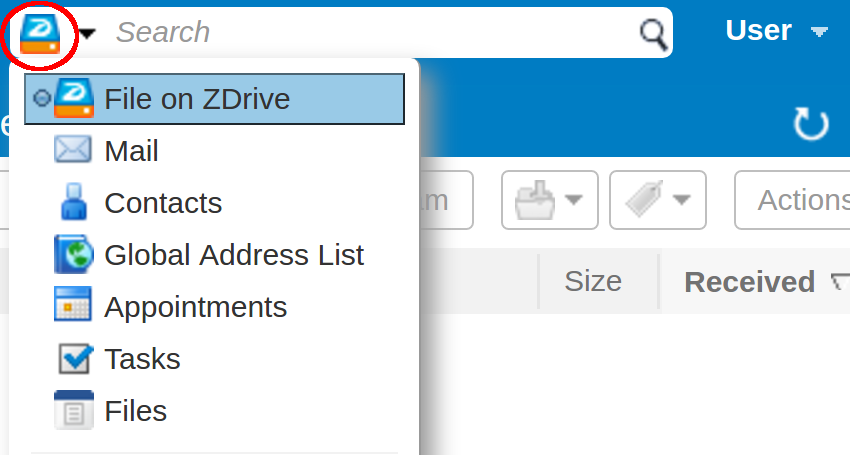
\includegraphics[scale=0.25]{\srcPath/images/ZD-searchMenu.png} 
\caption{Search Menu Item} 
\label{fig:searchMenu}
\end{figure}

The search feature has a 'string filter' and a 'location command'. 
Every search is threated as not case sensitive. \\
The string filter locates the files and the folders which names contains the string given (not case sensitive).
E.g: the results of the filter 'mp' can be "EXAMPLE.txt" and "Improvement.pdf".\\

The location command is in the following expression:
\begin{verbatim}
in:"/Documents"
\end{verbatim}
If the search is performed with just a 'location command', the results will be only the contents of the specific folder.\\

Any different search combination of multiple 'string filter' and a possible 'location command' returns 
the files and the folders matched in a recursive search.

\begin{warning}
    Multiple location commands are compared with an AND operator that makes them useless. Don't use them.
\end{warning}

